\chapter{Introduction}
\label{chap_intro}

\section{Motivation}
In the summer of 2015 I started to collaborate, as a volunteer, with the Mothers’ Milk Bank Northeast in Newton, MA. The milk bank is a small nonprofit that deals with the collection, processing and distribution of human milk.

This collaboration started completely by chance. I heard about the organization through an acquaintance and came for a visit. In that visit I learned about the story of the organization: Its vision, goals, methods and constraints. As a curious person, with a passion for understanding how things are done, I was intrigued. 

It was immediately clear that some of the challenges faced by the organization related to their unique operation and the lack of dedicated equipment in the market. With access to a machine shop at MIT and some basic fabrication skills, I felt like I could help. This resulted in an ongoing, fruitful collaboration. 

The collaboration benefited both sides. For me, this was a learning experience, a chance to utilize a newly acquired set of skills and, above all, make a real world impact. For the Milk Bank this was a chance to get a different perspective on their challenges, collaborate on solutions and raise awareness of their goals.   

Such asymmetry of knowledge and expertise between two groups or organizations, who would benefit from collaborating, is not unique. Established corporations bridge this gap by throwing resources, human and/or monetary, at it. For nonprofits and other organizations with fewer resources, that option is not available.

\marginpar {
  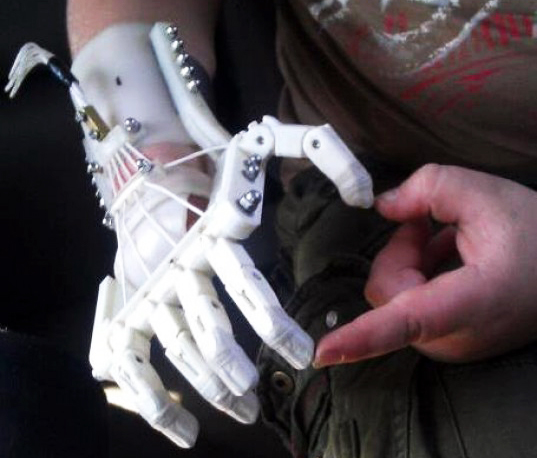
\includegraphics[width=\marginparwidth]{figures/robohand.jpg}
  A 3d printed prosthetic hand\cite{robohand} 
  \label{fig_enable}
} However, with recent improvements in technology and tools, hobbyist makers like myself are more capable than ever.  These makers are creating 3d printed prosthetics, Internet connected devices, and much more in their basements and community maker spaces. Collaborating with nonprofits allows these makers to practice their skills while making a difference. 

This thesis provides tools to facilitate these type of collaborations.


\section{Taxonomy}
In this thesis I propose a story centric distributed brainstorming and collaboration platform as a means to bridge the gap between makers and nonprofits. The following terms are used extensively throughout the thesis.

\begin{itemize}
\item \textit{Makers}:
The Maker movement is a relatively new subculture, an extension of the DIY (do it yourself) movement. It is comprised of individuals with passion for creating personalized physical objects in a non-commercial environment. These objects can be constructed using discarded equipment, digital fabrication tools such as 3d printers, or a combination of the above. I will further discuss the maker movement in the background chapter.

The individuals I write about in this thesis are indeed affiliated with the maker movement. However, I do not wish to limit the term maker to that alone. It is my belief that any capable volunteer, whether they're software developers, artists, or, God forbid, lawyers, can make significant impact. By doing so I choose to adopt the broad definition, yet somewhat obscure, of a maker as ``a person who makes something''. 

\item \textit{Nonprofits}: 
In this thesis I refer to nonprofits as the clients of the proposed platform. One example, The Mothers' Milk Bank Northeast is mentioned in the previous section. Nonprofit organizations are business entities which have a goal other than profit making. They often, though not always, suffer from shortages of funding and manpower. The nonprofits I discuss in this thesis will usually fall in that first category. With that said, it is completely plausible for other organizations or individuals, which seek help with their challenges to use this platform even without the official nonprofit title.

\item \textit{Story-centric}:
Derived from a story. A story in this case is one told by a nonprofit and describes their goals, methods, constraints and challenges. It is more broad and general than a solution specification or a problem statement. Nonprofits will often have this story well articulated, given that it serves as a tool in the ongoing quest for donations and volunteers. 

\item \textit{Brainstorming}:
A process in which a group of people attempts to work towards a solution of a problem by spontaneously suggesting ideas. 

\item \textit{Distributed Collaboration}:
In this thesis I refer to distributed collaboration as an ad-hoc collaboration, made over the Internet, between individuals who are not necessarily familiar with one another, or are affiliated in any way.  

\end{itemize}

\section{Goals}
In this thesis I wish to foster collaboration between the maker community and nonprofit organizations. I would like to expose makers to nonprofits and have them engage in collaboration. In doing so, makers can practice their skills, understand their value and have a real world impact. In turn, nonprofit can gain a different perspective on their challenges and collaborate towards solutions. 

\section{Contribution and Scope}
My thesis offers two primary contributions. First, I offer an outline for the process of story-centric brainstorming and collaboration. This outline will reflect my observations in participating in, witnessing and initiating these type of collaborations. Second, I will describe and implement a system that utilizes hypermedia as a medium for storytelling and allows for brainstorming and collaboration, based on the outlined process. The system will focus on the initial steps of collaboration: discovery, exploration and brainstorming. 

\section{Methodology} 
The main theme and a core principle of this thesis is co-design, an approach to design which attempts to actively involve all stakeholders. This approach is reflected both in the nature of collaborations discussed between makers and nonprofits and also in the research methodology itself, between myself and the different stakeholders. 

The outline of story centric brainstorming and collaboration, as presented in Chapter 3, is the product of on-site visits to the respective nonprofits, unstructured interviews, both with nonprofits and makers, and an ongoing dialog with the parties involved. 

\textit{This is How}, the web platform that facilitates distributed story-centric brainstorming and collaboration, was evaluated through structured interviews by the same nonprofits and makers in comparison to their experience in working on such collaborations in ``real life''. 

\section{Thesis Overview}

\begin{itemize}

\item Chapter \ref{chap_background} explores the background and related work of three of the main themes of this thesis: the maker movement, crowdsourcing systems and hypermedia.

\item Chapter \ref{chap_anatomy} provides an outline and discussion of story centric brainstorming and collaboration between makers and nonprofits through the prism of three case studies. 

\item Chapter \ref{chap_design} presents design considerations for adding a layer of distribution on top of the outline provided in Chapter 3. In it, I argue for the use of video as a medium for storytelling and discuss the main features of the proposed platform \textit{This is How}.

\item Chapter \ref{chap_impl} introduces the implementation for \textit{This is How}, covering both technology and user experience.  

\item Chapter \ref{chap_eval} presents an evaluation of \textit{This is How}, by means of comparison to ``real life'' collaborations, through structured interviews with the makers and nonprofits introduced previously in Chapter 3.

\item Chapter \ref{chap_conclusion} concludes the thesis, discusses limitations and future work, and includes personal reflections.      

\end{itemize}
